 \documentclass[12pt,a4paper]{article}
\usepackage{hyperref} % Use the Charter font for the document text
%\usepackage[UTF8]{ctex}
\usepackage{fullpage}
\usepackage{amsfonts,amssymb,amsmath}
\usepackage{mathtools}
\usepackage{tikz-cd}
\usepackage{tikz}
\usepackage{mathrsfs}
\usepackage{graphicx}
\usepackage{alltt}
\usepackage{amsfonts}
\usepackage{amsmath}
\usepackage{amssymb}
\usepackage{amsthm}
\usepackage{booktabs}
\usepackage{caption}
\usepackage{enumitem}
\usepackage{fancyhdr}
\usepackage{graphicx}
\usepackage{mathdots}
\usepackage{mathtools}
\usepackage{microtype}
\usepackage{multirow}
\usepackage{pdflscape}
\usepackage{pgfplots}
\usepackage{siunitx}
\usepackage{slashed}
\usepackage{tabularx}
\usepackage{slashed}

\usepackage{color}
\usepackage{tikz}
\usepackage{tkz-euclide}
\usepackage[normalem]{ulem}
\usepackage[all]{xy}
\usepackage{imakeidx}
\newcommand{\gc}{{\Gamma(M,C(M))}}
\newcommand{\n}{{\nabla}}
 \newcommand{\Gam}{\Gamma}
 
 
 
 \newcommand{\term}[1]{\textbf{#1}\index{#1}}

 
 
 
 \usetikzlibrary{decorations.markings}
\newcommand{\maplr}[2]{\begin{picture}(40,20)(0,20)
    \put(18,32){{\small $#1$}}
    \put(3,25){\vector(1,0){34}}
    \put(37,20){\vector(-1,0){34}}
     \put(18,10){{\small $#2$}}
  \end{picture}
}


%Caligraphic roman letters
\newcommand\calA{{\mathcal{A}}}
\newcommand\calB{{\mathcal{B}}}
\newcommand\calC{{\mathcal{C}}}
\newcommand\calD{{\mathcal{D}}}
\newcommand\calE{{\mathcal{E}}}
\newcommand\calF{{\mathcal{F}}}
\newcommand\calG{{\mathcal{G}}}
\newcommand\calH{{\mathcal{H}}}
\newcommand\calI{{\mathcal{I}}}
\newcommand\calJ{{\mathcal{J}}}
\newcommand\calK{{\mathcal{K}}}
\newcommand\calL{{\mathcal{L}}}
\newcommand\calM{{\mathcal{M}}}
\newcommand\calN{{\mathcal{N}}}
\newcommand\calO{{\mathcal{O}}}
\newcommand\calP{{\mathcal{P}}}
\newcommand\calQ{{\mathcal{Q}}}
\newcommand\calR{{\mathcal{R}}}
\newcommand\calS{{\mathcal{S}}}
\newcommand\calT{{\mathcal{T}}}
\newcommand\calU{{\mathcal{U}}}
\newcommand\calV{{\mathcal{V}}}
\newcommand\calW{{\mathcal{W}}}
\newcommand\calX{{\mathcal{X}}}
\newcommand\calY{{\mathcal{Y}}}
\newcommand\calZ{{\mathcal{Z}}}



%Bold roman letters
\newcommand\bfa{{\mathbf a}}            \newcommand\bfA{{\mathbf A}}
\newcommand\bfb{{\mathbf b}}            \newcommand\bfB{{\mathbf B}}
\newcommand\bfc{{\mathbf c}}            \newcommand\bfC{{\mathbf C}}
\newcommand\bfd{{\mathbf d}}            \newcommand\bfD{{\mathbf D}}
\newcommand\bfe{{\mathbf e}}            \newcommand\bfE{{\mathbf E}}
\newcommand\bff{{\mathbf f}}            \newcommand\bfF{{\mathbf F}}
\newcommand\bfg{{\mathbf g}}            \newcommand\bfG{{\mathbf G}}
\newcommand\bfh{{\mathbf h}}            \newcommand\bfH{{\mathbf H}}
\newcommand\bfi{{\mathbf i}}            \newcommand\bfI{{\mathbf I}}
\newcommand\bfj{{\mathbf j}}            \newcommand\bfJ{{\mathbf J}}
\newcommand\bfk{{\mathbf k}}            \newcommand\bfK{{\mathbf K}}
\newcommand\bfl{{\mathbf l}}            \newcommand\bfL{{\mathbf L}}
\newcommand\bfm{{\mathbf m}}            \newcommand\bfM{{\mathbf M}}
\newcommand\bfn{{\mathbf n}}            \newcommand\bfN{{\mathbf N}}
\newcommand\bfo{{\mathbf o}}            \newcommand\bfO{{\mathbf O}}
\newcommand\bfp{{\mathbf p}}            \newcommand\bfP{{\mathbf P}}
\newcommand\bfq{{\mathbf q}}            \newcommand\bfQ{{\mathbf Q}}
\newcommand\bfr{{\mathbf r}}            \newcommand\bfR{{\mathbf R}}
\newcommand\bfs{{\mathbf s}}            \newcommand\bfS{{\mathbf S}}
\newcommand\bft{{\mathbf t}}            \newcommand\bfT{{\mathbf T}}
\newcommand\bfu{{\mathbf u}}            \newcommand\bfU{{\mathbf U}}
\newcommand\bfv{{\mathbf v}}            \newcommand\bfV{{\mathbf V}}
\newcommand\bfw{{\mathbf w}}            \newcommand\bfW{{\mathbf W}}
\newcommand\bfx{{\mathbf x}}            \newcommand\bfX{{\mathbf X}}
\newcommand\bfy{{\mathbf y}}            \newcommand\bfY{{\mathbf Y}}
\newcommand\bfz{{\mathbf z}}            \newcommand\bfZ{{\mathbf Z}}

%Capital roman double letters
\newcommand\QQ{\mathbb{Q}}
\newcommand\WW{\mathbb{W}}
\newcommand\EE{\mathbb{E}}
\newcommand\RR{\mathbb{R}}
\newcommand\TT{\mathbb{T}}
\newcommand\YY{\mathbb{Y}}
\newcommand\UU{\mathbb{U}}
\newcommand\II{\mathbb{I}}
\newcommand\OO{\mathbb{O}}
\newcommand\PP{\mathbb{P}}
\renewcommand\AA{\mathbb{A}}
\renewcommand\SS{\mathbb{S}}
\newcommand\DD{\mathbb{D}}
\newcommand\FF{\mathbb{F}}
\newcommand\GG{\mathbb{G}}
\newcommand\HH{\mathbb{H}}
\newcommand\JJ{\mathbb{J}}
\newcommand\KK{\mathbb{K}}
\newcommand\LL{\mathbb{L}}
\newcommand\ZZ{\mathbb{Z}}
\newcommand\XX{\mathbb{X}}
\newcommand\CC{\mathbb{C}}
\newcommand\VV{\mathbb{V}}
\newcommand\BB{\mathbb{B}}
\newcommand\NN{\mathbb{N}}
\newcommand\MM{\mathbb{M}}


  %Euler Fraktur letters
\newcommand\grA{{\mathfrak{A}}} \newcommand\gra{{\mathfrak{a}}}
\newcommand\grB{{\mathfrak{B}}} \newcommand\grb{{\mathfrak{b}}}
\newcommand\grC{{\mathfrak{C}}} \newcommand\grc{{\mathfrak{c}}}
\newcommand\grD{{\mathfrak{D}}} \newcommand\grd{{\mathfrak{d}}}
\newcommand\grE{{\mathfrak{E}}} \newcommand\gre{{\mathfrak{e}}}
\newcommand\grF{{\mathfrak{F}}} \newcommand\grf{{\mathfrak{f}}}
\newcommand\grG{{\mathfrak{G}}} \newcommand\grg{{\mathfrak{g}}}
\newcommand\grH{{\mathfrak{H}}} \newcommand\grh{{\mathfrak{h}}}
\newcommand\grI{{\mathfrak{I}}} \newcommand\gri{{\mathfrak{i}}}
\newcommand\grJ{{\mathfrak{J}}} \newcommand\grj{{\mathfrak{j}}}
\newcommand\grK{{\mathfrak{K}}} \newcommand\grk{{\mathfrak{k}}}
\newcommand\grL{{\mathfrak{L}}} \newcommand\grl{{\mathfrak{l}}}
\newcommand\grM{{\mathfrak{M}}} \newcommand\grm{{\mathfrak{m}}}
\newcommand\grN{{\mathfrak{N}}} \newcommand\grn{{\mathfrak{n}}}
\newcommand\grO{{\mathfrak{O}}} \newcommand\gro{{\mathfrak{o}}}
\newcommand\grP{{\mathfrak{P}}} \newcommand\grp{{\mathfrak{p}}}
\newcommand\grQ{{\mathfrak{Q}}} \newcommand\grq{{\mathfrak{q}}}
\newcommand\grR{{\mathfrak{R}}} \newcommand\grr{{\mathfrak{r}}}
\newcommand\grS{{\mathfrak{S}}} \newcommand\grs{{\mathfrak{s}}}
\newcommand\grT{{\mathfrak{T}}} \newcommand\grt{{\mathfrak{t}}}
\newcommand\grU{{\mathfrak{U}}} \newcommand\gru{{\mathfrak{u}}}
\newcommand\grV{{\mathfrak{V}}} \newcommand\grv{{\mathfrak{v}}}
\newcommand\grW{{\mathfrak{W}}} \newcommand\grw{{\mathfrak{w}}}
\newcommand\grX{{\mathfrak{X}}} \newcommand\grx{{\mathfrak{x}}}
\newcommand\grY{{\mathfrak{Y}}} \newcommand\gry{{\mathfrak{y}}}
\newcommand\grZ{{\mathfrak{Z}}} \newcommand\grz{{\mathfrak{z}}}



\newcommand\nek{,\ldots,}
\newcommand\sdp{\times \hskip -0.3em {\raise 0.3ex
\hbox{$\scriptscriptstyle |$}}} % semidirect product

%words in roman font

\newcommand\area{\operatorname{area}}
\newcommand\Aug{\operatorname{Aug}}
\newcommand\Aut{\operatorname{Aut}}
\newcommand\Char{\operatorname{Char}}
\newcommand\Cl{\operatorname{Cl}}
\newcommand\cf{{\rm \,cf\,}}
\newcommand\Cone{\operatorname{Cone}}
\newcommand\cont{\operatorname{cont}}
\newcommand\codim{\operatorname{codim}}
\newcommand\conv{\operatorname{conv}}
\newcommand\Conv{\operatorname{Conv}}
\newcommand\const{\operatorname{const}}
\newcommand\Const{\operatorname{Const}}
\newcommand\Det{\operatorname{Det}}
\newcommand\diag{\operatorname{diag}}
\newcommand\diam{\operatorname{diam}}
\newcommand\Diam{\operatorname{Diam}}
\newcommand\dist{\operatorname{dist}}
\newcommand\Dom{\operatorname{Dom}}
\newcommand\dom{\operatorname{dom}}
\newcommand\End{\operatorname{End\,}}
\newcommand\Ext{\operatorname{Ext}}
\newcommand\esssup{\operatorname{ess\ sup}}
\newcommand\Ran{{\rm Ran}}
\newcommand\RANK{\operatorname{rank}}
\newcommand\Geo{\operatorname{Geo}}
\newcommand\GL{\operatorname{GL}}
\newcommand\Gr{\operatorname{Gr}}
\newcommand\gl{\operatorname{gl}}
\newcommand\grad{\mathop {\rm grad}}
\newcommand\Hom{\operatorname {Hom}}
\newcommand\im{\operatorname {im}}
\newcommand\IM{\operatorname{Im}}
\newcommand\Ind{\operatorname{Ind}}
\newcommand\ind{\operatorname{ind}}
\newcommand\Inf{\operatorname{Inf}}
\newcommand\Int{\operatorname{Int}}
\newcommand\Min{\operatorname{Min}}
\newcommand\MOD{\operatorname{mod}}
\newcommand{\Mor}{\operatorname{Mor}}
\newcommand{\Ob}{\operatorname{Ob\,}}
\newcommand\ord{\operatorname{ord}}
\newcommand\Ka{\operatorname{Ka}}
\newcommand\Ker{\operatorname{Ker}}
\newcommand\PGL{{\rm PGL}}
\newcommand\PGSp{{\rm PGSp}}
\newcommand\Plt{\operatorname{Plt}}
\newcommand\proj{\operatorname{proj}}
\newcommand\Proj{\operatorname{Proj}}
\newcommand\res{\rm res}
%\newcommand\rank{\rm rank}
\newcommand\rk{\operatorname{rk}}
\newcommand\Range{\operatorname{Range}}
\newcommand\RE{\operatorname{Re}}
\newcommand\Res{\operatorname{Res}}
\newcommand\rot{\operatorname{rot}}
\newcommand\Max{\operatorname{Max}}
\newcommand\Maximum{\operatorname{Maximum}}
\newcommand\Minimum{\operatorname{Minimum}}
\newcommand\Minimize{\operatorname{Minimize}}
\newcommand\Prob{\operatorname{Prob}}
\newcommand\sech{\rm sech}
\newcommand\sgn{\operatorname{sgn}}
\newcommand{\sign}{\operatorname{sign}}
\newcommand\SL{{\rm SL}}
\newcommand\Sbm{\operatorname{Sbm}}
\newcommand\SO{{\rm SO}}
\newcommand\SPAN{\operatorname{span}}
\newcommand\spin{\operatorname{spin}}
\newcommand\spec{{\rm spec}}
\newcommand\supess{\operatorname{sup\ ess}}
\newcommand\supp{\operatorname{supp}}
\newcommand\Supp{\operatorname{Supp}}
\newcommand\Sup{\operatorname{Sup}}
\newcommand\Sym{\operatorname{Sym}}
\newcommand\tr{\operatorname{tr}}
\newcommand\Tr{\operatorname{Tr}}
\newcommand\Tor{\operatorname{Tor}}
\newcommand\Var{\operatorname{Var}}
\newcommand\Vol{\operatorname{Vol}}
%\newcommand\vol{\operatorname{vol}}

%overlined math alphabet
\newcommand\oa{{\overline{a}}}
\newcommand\oA{{\overline{A}}}
\newcommand\ob{{\overline{b}}}
\newcommand\oB{{\overline{B}}}
\newcommand\oc{{\overline{c}}}
\newcommand\oC{{\overline{C}}}
\newcommand\oD{{\overline{D}}}
\newcommand\od{{\overline{d}}}
\newcommand\oE{{\overline{E}}}
\renewcommand\oe{{\overline{e}}}
\newcommand\of{{\overline{f}}}
\newcommand\oF{{\overline{F}}}
\newcommand\og{{\overline{g}}}
\newcommand\oG{{\overline{G}}}
\newcommand\oh{{\overline{h}}}
\newcommand\oH{{\overline{H}}}
\newcommand\oI{{\overline{I}}}
\newcommand\oj{{\overline{j}}}
\newcommand\oJ{{\overline{J}}}
\newcommand\ok{{\overline{k}}}
\newcommand\oK{{\overline{K}}}
\newcommand\oL{{\overline{L}}}
\newcommand\om{{\overline{m}}}
\newcommand\oM{{\overline{M}}}
\newcommand\oN{{\overline{N}}}
\newcommand\oO{{\overline{O}}}
\newcommand\oo{{\overline{o}}}
\newcommand\op{{\overline{p}}}
\newcommand\oP{{\overline{P}}}
\newcommand\oq{{\overline{q}}}
\newcommand\oQ{{\overline{Q}}}
\newcommand\OR{{\overline{r}}}
\newcommand\oS{{\overline{S}}}
\newcommand\os{{\overline{s}}}
\newcommand\ot{{\overline{t}}}
\newcommand\oT{{\overline{T}}}
\newcommand\ou{{\overline{u}}}
\newcommand\oU{{\overline{U}}}
\newcommand\ov{{\overline{v}}}
\newcommand\oV{{\overline{V}}}
\newcommand\ow{{\overline{w}}}
\newcommand\oW{{\overline{W}}}
\newcommand\ox{{\overline{x}}}
\newcommand\oX{{\overline{X}}}
\newcommand\oy{{\overline{y}}}
\newcommand\oY{{\overline{Y}}}
\newcommand\oz{{\overline{z}}}
\newcommand\oZ{{\overline{Z}}}

%overlined Greek alphabet
\newcommand\oalp{{\overline{\alpha}}}
\newcommand\obet{{\overline{\bet}}}
\newcommand\odel{{\overline{\del}}}
\newcommand\oDel{{\overline{\Del}}}
\newcommand\ocup{{\overline{\cup}}}
\newcommand\ovarphi{{\overline{\varphi}}}
\newcommand\ochi{{\overline{\chi}}}
\newcommand\oeps{{\overline{\eps}}}
\newcommand\oeta{{\overline{\eta}}}
\newcommand\ogam{{\overline{\gam}}}
\newcommand\okap{{\overline{\kap}}}
\newcommand\olam{{\overline{\lambda}}}
\newcommand\oLam{{\overline{\Lambda}}}
\newcommand\omu{{\overline{\mu}}}
\newcommand\onu{{\overline{\nu}}}
\newcommand\oOme{{\overline{\Ome}}}
\newcommand\ophi{\overline{\phi}}
\newcommand\oPhi{{\overline{\Phi}}}
\newcommand\opi{{\overline{\pi}}}
\newcommand\oPsi{{\overline{\Psi}}}
\newcommand\opsi{{\overline{\psi}}}
\newcommand\orho{{\overline{\rho}}}
\newcommand\osig{{\overline{\sig}}}
\newcommand\otau{{\overline{\tau}}}
\newcommand\otet{{\overline{\theta}}}
\newcommand\oxi{{\overline{\xi}}}
\newcommand\oome{\overline{\ome}}
\newcommand\opart{{\overline{\partial}}}


%underlined math alphabet
\newcommand\ua{{\underline{a}}}
\newcommand\ub{{\underline{b}}}
\newcommand\uc{{\underline{c}}}
\newcommand\uD{{\underline{D}}}
\newcommand\uk{{\underline{k}}}
\newcommand\ue{{\underline{e}}}
\newcommand\uj{{\underline{j}}}
\newcommand\ul{{\underline{l}}}
\newcommand\uL{{\underline{L}}}
\newcommand\uo{{\underline{o}}}
\newcommand\uO{{\underline{O}}}
\newcommand\uP{{\underline{P}}}
\newcommand\uQ{{\underline{Q}}}
\newcommand\um{{\underline{m}}}
\newcommand\uM{{\underline{M}}}
\newcommand\un{{\underline{n}}}
\newcommand\us{{\underline{s}}}
\newcommand\ut{{\underline{t}}}
\newcommand\uu{{\underline{u}}}
\newcommand\uv{{\underline{v}}}
\newcommand\uV{{\underline{V}}}
\newcommand\ux{{\underline{x}}}
\newcommand\uX{{\underline{X}}}
\newcommand\uy{{\underline{y}}}
\newcommand\uz{{\underline{z}}}

%underline Greek alphabet
\newcommand\ualp{{\underline{\alp}}}
\newcommand\ubet{{\underline{\bet}}}
\newcommand\uchi{{\underline{\chi}}}
\newcommand\udel{{\underline{\del}}}
\newcommand\uell{{\underline{\ell}}}
\newcommand\ueps{{\underline{\eps}}}
\newcommand\ueta{{\underline{\eta}}}
\newcommand\uGam{{\underline{\Gamma}}}
\newcommand\unu{{\underline{\nu}}}
\newcommand\uome{{\underline{\omega}}}
\newcommand\utet{{\underline{\tet}}}
\newcommand\ulam{{\underline{\lam}}}


%math alphabet with hat
\newcommand\hata{{\widehat{a}}}
\newcommand\hatA{{\widehat{A}}}
\newcommand\hatb{{\widehat{b}}}
\newcommand\hatc{{\widehat{c}}}
\newcommand\hatC{{\widehat{C}}}
\newcommand\hatB{{\widehat{B}}}
\newcommand\hatD{{\widehat{D}}}
\newcommand\hate{{\widehat{e}}}
\newcommand\hatE{{\widehat{E}}}
\newcommand\hatf{{\widehat{f}}}
\newcommand\hatF{{\widehat{F}}}
\newcommand\hatg{{\widehat{g}}}
\newcommand\hatG{{\widehat{G}}}
\newcommand\hath{{\widehat{h}}}
\newcommand\hatH{{\widehat{H}}}
\newcommand\hati{{\hat{i}}}
\newcommand\hatI{{\hat{I}}}
\newcommand\hatj{{\widehat{j}}}
\newcommand\hatJ{{\widehat{J}}}
\newcommand\hatk{{\widehat{k}}}
\newcommand\hatK{{\widehat{K}}}
\newcommand\hatL{{\widehat{L}}}
\newcommand\hatm{{\widehat{m}}}
\newcommand\hatM{{\widehat{M}}}
\newcommand\hatn{{\widehat{n}}}
\newcommand\hatN{{\widehat{N}}}
\newcommand\hatp{{\widehat{p}}}
\newcommand\hatP{{\widehat{P}}}
\newcommand\hatr{{\widehat{r}}}
\newcommand\hatR{{\widehat{R}}}
\newcommand\hatq{{\widehat{q}}}
\newcommand\hatQ{{\widehat{Q}}}
\newcommand\hatT{{\widehat{T}}}
\newcommand\hatu{{\widehat{u}}}
\newcommand\hatU{{\widehat{U}}}
\newcommand\hatV{{\widehat{V}}}
\newcommand\hatv{{\widehat{v}}}
\newcommand\hatw{{\widehat{w}}}
\newcommand\hatW{{\widehat{W}}}
\newcommand\hatx{{\widehat{x}}}
\newcommand\hatX{{\widehat{X}}}
\newcommand\haty{{\widehat{y}}}
\newcommand\hatY{{\widehat{Y}}}
\newcommand\hatZ{{\widehat{Z}}}
\newcommand\hatz{{\widehat{z}}}

%Greek alphabet with hat
\newcommand\hatalp{{\widehat{\alpha}}}
\newcommand\hatdel{{\widehat{\delta}}}
\newcommand\hatDel{{\widehat{\Delta}}}
\newcommand\hatbet{{\widehat{\beta}}}
\newcommand\hateps{{\hat{\eps}}}
\newcommand\hatgam{{\widehat{\gamma}}}
\newcommand\hatGam{{\widehat{\Gamma}}}
\newcommand\hatlam{{\widehat{\lambda}}}
\newcommand\hatmu{{\widehat{\mu}}}
\newcommand\hatnu{{\widehat{\nu}}}
\newcommand\hatOme{{\widehat{\Ome}}}
\newcommand\hatphi{{\widehat{\phi}}}
\newcommand\hatPhi{{\widehat{\Phi}}}
\newcommand\hatpi{{\widehat{\pi}}}
\newcommand\hatpsi{{\widehat{\psi}}}
\newcommand\hatPsi{{\widehat{\Psi}}}
\newcommand\hatrho{{\widehat{\rho}}}
\newcommand\hatsig{{\widehat{\sig}}}
\newcommand\hatSig{{\widehat{\Sig}}}
\newcommand\hattau{{\widehat{\tau}}}
\newcommand\hattet{{\widehat{\theta}}}
\newcommand\hatvarphi{{\widehat{\varphi}}}
\newcommand\hatZZ{{\widehat{\ZZ}}}


%roman with widetilde

\newcommand\tilA{{\widetilde{A}}}
\newcommand\tila{{\widetilde{a}}}
\newcommand\tilB{{\widetilde{B}}}
\newcommand\tilb{{\widetilde{b}}}
\newcommand\tilc{{\widetilde{c}}}
\newcommand\tilC{{\widetilde{C}}}
\newcommand\tild{{\widetilde{d}}}
\newcommand\tilD{{\widetilde{D}}}
\newcommand\tilE{{\widetilde{E}}}
\newcommand\tilf{{\widetilde{f}}}
\newcommand\tilF{{\widetilde{F}}}
\newcommand\tilg{{\widetilde{g}}}
\newcommand\tilG{{\widetilde{G}}}
\newcommand\tilh{{\widetilde{h}}}
\newcommand\tilk{{\widetilde{k}}}
\newcommand\tilK{{\widetilde{K}}}
\newcommand\tilj{{\widetilde{j}}}
\newcommand\tilJ{{\widetilde{J}}}
\newcommand\tilm{{\widetilde{m}}}
\newcommand\tilM{{\widetilde{M}}}
\newcommand\tilH{{\widetilde{H}}}
\newcommand\tilL{{\widetilde{L}}}
\newcommand\tilN{{\widetilde{N}}}
\newcommand\tiln{{\widetilde{n}}}
\newcommand\tilO{{\widetilde{O}}}
\newcommand\tilP{{\widetilde{P}}}
\newcommand\tilp{{\widetilde{p}}}
\newcommand\tilq{{\widetilde{q}}}
\newcommand\tilQ{{\widetilde{Q}}}
\newcommand\tilR{{\widetilde{R}}}
\newcommand\tilr{{\widetilde{r}}}
\newcommand\tilS{{\widetilde{S}}}
\newcommand\tils{{\widetilde{s}}}
\newcommand\tilT{{\widetilde{T}}}
\newcommand\tilt{{\widetilde{t}}}
\newcommand\tilu{{\widetilde{u}}}
\newcommand\tilU{{\widetilde{U}}}
\newcommand\tilv{{\widetilde{v}}}
\newcommand\tilV{{\widetilde{V}}}
\newcommand\tilw{{\widetilde{w}}}
\newcommand\tilW{{\widetilde{W}}}
\newcommand\tilX{{\widetilde{X}}}
\newcommand\tilx{{\widetilde{x}}}
\newcommand\tily{{\widetilde{y}}}
\newcommand\tilY{{\widetilde{Y}}}
\newcommand\tilZ{{\widetilde{Z}}}
\newcommand\tilz{{\widetilde{z}}}

%Greek alphabet with widetilde
\newcommand\tilalp{{\widetilde{\alpha}}}
\newcommand\tilbet{{\widetilde{\beta}}}
\newcommand\tildel{{\widetilde{\delta}}}
\newcommand\tilDel{{\widetilde{\Delta}}}
\newcommand\tilchi{{\widetilde{\chi}}}
\newcommand\tileps{{\widetilde{\eps}}}
\newcommand\tileta{{\widetilde{\eta}}}
\newcommand\tilgam{{\widetilde{\gamma}}}
\newcommand\tilGam{{\widetilde{\Gamma}}}
\newcommand\tilome{{\widetilde{\ome}}}
\newcommand\tillam{{\widetilde{\lam}}}
\newcommand\tilmu{{\widetilde{\mu}}}
\newcommand\tilphi{{\widetilde{\phi}}}
\newcommand\tilpi{{\widetilde{\pi}}}
\newcommand\tilpsi{{\widetilde{\psi}}}
\renewcommand\tilome{{\widetilde{\ome}}}
\newcommand\tilOme{{\widetilde{\Ome}}}
\newcommand\tilPhi{{\widetilde{\Phi}}}
\newcommand\tilQQ{{\widetilde{\QQ}}}
\newcommand\tilrho{{\widetilde{\rho}}}
\newcommand\tilsig{{\widetilde{\sig}}}
\newcommand\tiltau{{\widetilde{\tau}}}
\newcommand\tiltet{{\widetilde{\theta}}}
\newcommand\tilvarphi{{\widetilde{\varphi}}}
\newcommand\tilxi{{\widetilde{\xi}}}



\newcommand{\bea}{\begin{eqnarray*}}
\newcommand{\eea}{\end{eqnarray*}}

\newcommand{\bA}{\ensuremath{\mathbb{A}}}
\newcommand{\bB}{\ensuremath{\mathbb{B}}}
\newcommand{\bC}{\ensuremath{\mathbb{C}}}
\newcommand{\bD}{\ensuremath{\mathbb{D}}}
\newcommand{\bE}{\ensuremath{\mathbb{E}}}
\newcommand{\bF}{\ensuremath{\mathbb{F}}}
\newcommand{\bG}{\ensuremath{\mathbb{G}}}
\newcommand{\bH}{\ensuremath{\mathbb{H}}}
\newcommand{\bI}{\ensuremath{\mathbb{I}}}
\newcommand{\bJ}{\ensuremath{\mathbb{J}}}
\newcommand{\bK}{\ensuremath{\mathbb{K}}}
\newcommand{\bL}{\ensuremath{\mathbb{L}}}
\newcommand{\bM}{\ensuremath{\mathbb{M}}}
\newcommand{\bN}{\ensuremath{\mathbb{N}}}
\newcommand{\bO}{\ensuremath{\mathbb{O}}}
\newcommand{\bP}{\ensuremath{\mathbb{P}}}
\newcommand{\bQ}{\ensuremath{\mathbb{Q}}}
\newcommand{\bR}{\ensuremath{\mathbb{R}}}
\newcommand{\bS}{\ensuremath{\mathbb{S}}}
\newcommand{\bT}{\ensuremath{\mathbb{T}}}
\newcommand{\bU}{\ensuremath{\mathbb{U}}}
\newcommand{\bV}{\ensuremath{\mathbb{V}}}
\newcommand{\bW}{\ensuremath{\mathbb{W}}}
\newcommand{\bX}{\ensuremath{\mathbb{X}}}
\newcommand{\bY}{\ensuremath{\mathbb{Y}}}
\newcommand{\bZ}{\ensuremath{\mathbb{Z}}}


%
%\parskip=1em
%\parindent=0.3in
%\setlength\oddsidemargin{0.5in} \setlength\evensidemargin{0.5in}
%\setlength\textwidth{5.5in}
%
%\hfuzz6pt % Don't bother to report over-full boxes if over-edge is < 6pt
%
%\newlength{\defbaselineskip}
%\setlength{\defbaselineskip}{\baselineskip}
%\newcommand{\setlinespacing}[1]%
%           {\setlength{\baselineskip}{#1 \defbaselineskip}}
%\newcommand{\doublespacing}{\setlength{\baselineskip}%
%                           {2.0 \defbaselineskip}}
%\newcommand{\singlespacing}{\setlength{\baselineskip}{\defbaselineskip}}
%
%\newcommand{\properpagestyle}{\pagestyle{myheadings}\markboth{}{}\markright{}}




%\def\Ric{\mathop{\rm Ric}}
%\def\cRic{\mathop{\stackrel{\circ}{\Ric}}}
%\def\Scal{\mathop{\rm R}}
%\def\scL{\mathop{\mathcal L}}
%\def\Hess{\mathop{\rm Hess}}
%\def\bt{\mathop{\bar\tau}}
%\def\dist{\mathop{\rm dist}}
%\def\Cut{\mathop{\rm Cut}}
%\def\Riem{\mathop{\rm Rm}}
%\def\scal{\mathop{\rm scal}}
%\def\Sec{\mathop{\rm Sec}}
%\def\Diam{\mathop{\rm Diam}}
%\def\CS{\mathop{\rm C_S}}
%\def\V{\mathop{\rm V}}
%\def\Vol{\mathop{\rm Vol}}
%\def\Area{\mathop{\rm Area}}
%\def\VR{\mathop{\rm VR}}
%\def\supp{\mathop{\rm supp}}
%\def\div{\mathop{\rm div}}
%\def\inj{\mathop{\rm inj}}
%\def\diam{\mathop{\rm diam}}
%\def\Id{\mathop{\rm Id}}
%\def\RRR{\mathop{\mathcal{R}}}
%\def\MMM{\mathop{\mathcal{M}}}
%\def\HHH{\mathop{\mathcal{H}}}
%\def\VVV{\mathop{\mathcal{V}}}
%\def\FF{\mathop{\mathbb{F}}}
%\def\RR{\mathop{\mathbb{R}}}
%\def\QQ{\mathop{\mathbb{Q}}}
%\def\CC{\mathop{\mathbb{C}}}
%\def\ZZ{\mathop{\mathbb{Z}}}
%\def\SS{\mathop{\mathbb{S}}}
%\def\SSS{\mathop{\mathcal{S}}}
%\def\PP{\mathop{\mathbb{P}}}
%\def\End{\mathop{\rm End}}
%\def\Aut{\mathop{\rm Aut}}
%\def\Ad{\mathop{\rm Ad}}
%\def\ad{\mathop{\rm ad}}
%\def\hht{\mathop{\rm ht}}
%\def\gl{\mathop{\mathfrak{gl}}}
%\def\ssl{\mathop{\mathfrak{sl}}}
%\def\TP{\mathop{\mathcal{TP}}}
%\def\PPP{\mathop{\mathcal{P}}}
%\def\gggg{\mathop{\mathfrak{g}}}
%\def\ffff{\mathop{\mathfrak{f}}}
%\def\OO{\mathop{\mathcal{O}}}
%\def\oo{\mathop{\mathfrak{o}}}
%\def\GG{\mathop{\mathcal{G}}}
%\def\WWW{\mathop{\mathcal{W}}}
%\def\Rad{\mathop{\rm Rad}}
%\def\Der{\mathop{\rm Der}}
%\def\Ker{\mathop{\rm Ker}}
%\def\Im{\mathop{\rm Im}}
%\def\ind{\mathop{\rm ind}}


\def\be{\begin{eqnarray*}}
\def\ee{\end{eqnarray*}}
\def\beg{\begin{eqnarray*}}
\def\ees{\end{eqnarray*}}


%\newcommand{\qed}{\hfill$\Box$}
\theoremstyle{definition}
\newtheorem*{aim}{Aim}
\newtheorem*{axiom}{Axiom}
\newtheorem*{claim}{Claim}
\newtheorem*{cor}{Corollary}
\newtheorem*{conjecture}{Conjecture}
\newtheorem*{defi}{Definition}
\newtheorem*{eg}{Example}
\newtheorem*{ex}{Exercise}
\newtheorem*{fact}{Fact}
\newtheorem*{law}{Law}
\newtheorem*{lemma}{Lemma}
\newtheorem*{notation}{Notation}
\newtheorem*{prop}{Proposition}
\newtheorem*{question}{Question}
\newtheorem*{thm}{Theorem}





% Maths symbols
\newcommand{\abs}[1]{\left\lvert #1\right\rvert}
%\newcommand\ad{\mathrm{ad}}
\newcommand\AND{\mathsf{AND}}
\newcommand\Art{\mathrm{Art}}
\newcommand{\Bilin}{\mathrm{Bilin}}
\newcommand{\bket}[1]{\left\lvert #1\right\rangle}
\newcommand{\B}{\mathcal{B}}
\newcommand{\bolds}[1]{{\bfseries #1}}
\newcommand{\brak}[1]{\left\langle #1 \right\rvert}
\newcommand{\braket}[2]{\left\langle #1\middle\vert #2 \right\rangle}
\newcommand{\bra}{\langle}
\newcommand{\cat}[1]{\mathsf{#1}}
\newcommand{\C}{\mathbb{C}}
\newcommand{\CP}{\mathbb{CP}}
\newcommand{\cU}{\mathcal{U}}
%\newcommand{\Der}{\mathrm{Der}}
\newcommand{\D}{\mathrm{D}}
\newcommand{\dR}{\mathrm{dR}}
\newcommand{\E}{\mathbb{E}}
\newcommand{\F}{\mathbb{F}}
\newcommand{\Frob}{\mathrm{Frob}}
%\newcommand{\GG}{\mathbb{G}}
%\newcommand{\gl}{\mathfrak{gl}}
%\newcommand{\GL}{\mathrm{GL}}
\newcommand{\G}{\mathcal{G}}
%\newcommand{\Gr}{\mathrm{Gr}}
\newcommand{\haut}{\mathrm{ht}}
\newcommand{\Hol}{\mathrm{Hol}}
\newcommand{\hol}{\mathfrak{hol}}
%\newcommand{\Id}{\mathrm{Id}}
\newcommand{\ket}{\rangle}
\newcommand{\lie}[1]{\mathfrak{#1}}
\newcommand{\Mat}{\mathrm{Mat}}
\newcommand{\N}{\mathbb{N}}
\newcommand{\norm}[1]{\left\lVert #1\right\rVert}
\newcommand{\normalorder}[1]{\mathop{:}\nolimits\!#1\!\mathop{:}\nolimits}
\newcommand{\NOT}{\mathsf{NOT}}
%\newcommand{\op}{\mathrm{op}}
\newcommand{\Oc}{\mathcal{O}}
\newcommand{\Or}{\mathrm{O}}
%%\newcommand\OR{\mathsf{OR}}
%\newcommand{\ort}{\mathfrak{o}}
%\newcommand{\PGL}{\mathrm{PGL}}
%\newcommand{\ph}{\,\cdot\,}
%\newcommand{\pr}{\mathrm{pr}}
%\newcommand{\Prob}{\mathbb{P}}
%\newcommand{\PSL}{\mathrm{PSL}}
%\newcommand{\Ps}{\mathcal{P}}
%\newcommand{\PSU}{\mathrm{PSU}}
%\newcommand{\pt}{\mathrm{pt}}
%\newcommand{\qeq}{\mathrel{``{=}"}}
%\newcommand{\Q}{\mathbb{Q}}
%\newcommand{\R}{\mathbb{R}}
%\newcommand{\RP}{\mathbb{RP}}
%\newcommand{\Rs}{\mathcal{R}}
%\newcommand{\SL}{\mathrm{SL}}
%\newcommand{\so}{\mathfrak{so}}
%\newcommand{\SO}{\mathrm{SO}}
%\newcommand{\Spin}{\mathrm{Spin}}
%\newcommand{\Sp}{\mathrm{Sp}}
%\newcommand{\su}{\mathfrak{su}}
%\newcommand{\SU}{\mathrm{SU}}
%\newcommand{\term}[1]{\textbf{#1}\index{#1}}
%\newcommand{\T}{\mathbb{T}}
%\newcommand{\tv}[1]{|#1|}
%\newcommand{\U}{\mathrm{U}}
%\newcommand{\uu}{\mathfrak{u}}
%\newcommand{\Vect}{\mathrm{Vect}}
%\newcommand{\wsto}{\stackrel{\mathrm{w}^*}{\to}}
%\newcommand{\wt}{\mathrm{wt}}
%\newcommand{\wto}{\stackrel{\mathrm{w}}{\to}}
%\newcommand{\Z}{\mathbb{Z}}
%\renewcommand{\d}{\mathrm{d}}
%\renewcommand{\H}{\mathbb{H}}
%\renewcommand{\P}{\mathbb{P}}
%\renewcommand{\sl}{\mathfrak{sl}}
%\renewcommand{\vec}[1]{\boldsymbol{\mathbf{#1}}}
%%\renewcommand{\F}{\mathcal{F}}

\def\sm{\mathop{C^\infty}}


\let\Im\relax
\let\Re\relax

\DeclareMathOperator{\adj}{adj}
\DeclareMathOperator{\Ann}{Ann}
%\DeclareMathOperator{\area}{area}
%\DeclareMathOperator{\Aut}{Aut}
\DeclareMathOperator{\Bernoulli}{Bernoulli}
\DeclareMathOperator{\betaD}{beta}
\DeclareMathOperator{\bias}{bias}
\DeclareMathOperator{\binomial}{binomial}
\DeclareMathOperator{\card}{card}
\DeclareMathOperator{\ccl}{ccl}
%\DeclareMathOperator{\Char}{char}
\DeclareMathOperator{\ch}{ch}
\DeclareMathOperator{\cl}{cl}
\DeclareMathOperator{\cls}{\overline{\mathrm{span}}}
\DeclareMathOperator{\coker}{coker}
%\DeclareMathOperator{\conv}{conv}
\DeclareMathOperator{\corr}{corr}
\DeclareMathOperator{\cosec}{cosec}
\DeclareMathOperator{\cosech}{cosech}
\DeclareMathOperator{\cov}{cov}
\DeclareMathOperator{\covol}{covol}
%\DeclareMathOperator{\diag}{diag}
%\DeclareMathOperator{\diam}{diam}
\DeclareMathOperator{\Diff}{Diff}
\DeclareMathOperator{\disc}{disc}
%\DeclareMathOperator{\dom}{dom}
%\DeclareMathOperator{\End}{End}
\DeclareMathOperator{\energy}{energy}
\DeclareMathOperator{\erfc}{erfc}
\DeclareMathOperator{\erf}{erf}
%\DeclareMathOperator*{\esssup}{ess\,sup}
\DeclareMathOperator{\ev}{ev}
%\DeclareMathOperator{\Ext}{Ext}
\DeclareMathOperator{\fst}{fst}
\DeclareMathOperator{\Fit}{Fit}
\DeclareMathOperator{\fix}{fix}
\DeclareMathOperator{\Frac}{Frac}
\DeclareMathOperator{\Gal}{Gal}
\DeclareMathOperator{\gammaD}{gamma}
\DeclareMathOperator{\gr}{gr}
\DeclareMathOperator{\hcf}{hcf}
%\DeclareMathOperator{\Hom}{Hom}
\DeclareMathOperator{\id}{id}
\DeclareMathOperator{\Image}{image}
\DeclareMathOperator{\Im}{Im}
%\DeclareMathOperator{\Ind}{Ind}
%\DeclareMathOperator{\Int}{Int}
%\DeclareMathOperator{\Isom}{Isom}
%\DeclareMathOperator{\lcm}{lcm}
%\DeclareMathOperator{\length}{length}
%\DeclareMathOperator{\Lie}{Lie}
%\DeclareMathOperator{\like}{like}
%\DeclareMathOperator{\Lk}{Lk}
%\DeclareMathOperator{\Maps}{Maps}
%\DeclareMathOperator{\mse}{mse}
%\DeclareMathOperator{\multinomial}{multinomial}
%\DeclareMathOperator{\orb}{orb}
%\DeclareMathOperator{\ord}{ord}
%\DeclareMathOperator{\otp}{otp}
%\DeclareMathOperator{\Poisson}{Poisson}
%\DeclareMathOperator{\poly}{poly}
%\DeclareMathOperator{\rank}{rank}
%\DeclareMathOperator{\rel}{rel}
%%\DeclareMathOperator{\Rad}{Rad}
%\DeclareMathOperator{\Re}{Re}
%\DeclareMathOperator*{\res}{res}
%\DeclareMathOperator{\Res}{Res}
%%\DeclareMathOperator{\Ric}{Ric}
%\DeclareMathOperator{\rk}{rk}
%\DeclareMathOperator{\Rees}{Rees}
%\DeclareMathOperator{\Root}{Root}
%\DeclareMathOperator{\sech}{sech}
%\DeclareMathOperator{\sgn}{sgn}
%\DeclareMathOperator{\snd}{snd}
%\DeclareMathOperator{\Spec}{Spec}
%\DeclareMathOperator{\spn}{span}
%\DeclareMathOperator{\stab}{stab}
%\DeclareMathOperator{\St}{St}
%%\DeclareMathOperator{\supp}{supp}
%\DeclareMathOperator{\Syl}{Syl}
%\DeclareMathOperator{\Sym}{Sym}
%\DeclareMathOperator{\tr}{tr}
%\DeclareMathOperator{\Tr}{Tr}
%\DeclareMathOperator{\var}{var}
%\DeclareMathOperator{\vol}{vol}
%\usetikzlibrary{knots}




\pgfarrowsdeclarecombine{twolatex'}{twolatex'}{latex'}{latex'}{latex'}{latex'}
\tikzset{->/.style = {decoration={markings,
                                  mark=at position 1 with {\arrow[scale=2]{latex'}}},
                      postaction={decorate}}}
\tikzset{<-/.style = {decoration={markings,
                                  mark=at position 0 with {\arrowreversed[scale=2]{latex'}}},
                      postaction={decorate}}}
\tikzset{<->/.style = {decoration={markings,
                                   mark=at position 0 with {\arrowreversed[scale=2]{latex'}},
                                   mark=at position 1 with {\arrow[scale=2]{latex'}}},
                       postaction={decorate}}}
\tikzset{->-/.style = {decoration={markings,
                                   mark=at position #1 with {\arrow[scale=2]{latex'}}},
                       postaction={decorate}}}
\tikzset{-<-/.style = {decoration={markings,
                                   mark=at position #1 with {\arrowreversed[scale=2]{latex'}}},
                       postaction={decorate}}}
\tikzset{->>/.style = {decoration={markings,
                                  mark=at position 1 with {\arrow[scale=2]{latex'}}},
                      postaction={decorate}}}
\tikzset{<<-/.style = {decoration={markings,
                                  mark=at position 0 with {\arrowreversed[scale=2]{twolatex'}}},
                      postaction={decorate}}}
\tikzset{<<->>/.style = {decoration={markings,
                                   mark=at position 0 with {\arrowreversed[scale=2]{twolatex'}},
                                   mark=at position 1 with {\arrow[scale=2]{twolatex'}}},
                       postaction={decorate}}}
\tikzset{->>-/.style = {decoration={markings,
                                   mark=at position #1 with {\arrow[scale=2]{twolatex'}}},
                       postaction={decorate}}}
\tikzset{-<<-/.style = {decoration={markings,
                                   mark=at position #1 with {\arrowreversed[scale=2]{twolatex'}}},
                       postaction={decorate}}}


\tikzset{circ/.style = {fill, circle, inner sep = 0, minimum size = 3}}
\tikzset{scirc/.style = {fill, circle, inner sep = 0, minimum size = 1.5}}
\tikzset{mstate/.style={circle, draw, blue, text=black, minimum width=0.7cm}}

\tikzset{eqpic/.style={baseline={([yshift=-.5ex]current bounding box.center)}}}
\tikzset{commutative diagrams/.cd,cdmap/.style={/tikz/column 1/.append style={anchor=base east},/tikz/column 2/.append style={anchor=base west},row sep=tiny}}


\definecolor{mblue}{rgb}{0.2, 0.3, 0.8}
\definecolor{morange}{rgb}{1, 0.5, 0}
\definecolor{mgreen}{rgb}{0.1, 0.4, 0.2}
\definecolor{mred}{rgb}{0.5, 0, 0}


%\title{ Lecture 4}
\begin{document}\thispagestyle{empty}

\centerline{\Large \bf Lecture 12}

\centerline{\Large \bf  Nakahara section 12}


\section{Index Theorem}

Finally, we will study celebrated \term{Atiyah-Singer index theorem}. The index theorem states the equivalence between the index of an elliptic operator $D$, which is analytic object, and the characteristic classes, which are topological object. This theorem is one of milestones in mathematics of 20th century. The index theorem plays a crucial role in physics like anomaly, fermion zero modes and supersymmetry. In fact, in the tasteful book \cite{index-book}, you can feel excitement when the index theorem has been formulated. I highly recommend you to read this book.

\subsection{Symbol, elliptic operator, analytic index}

Let $E$ and $F$ be vector bundles of rank $m$ over an $n$-dimensional $M$.
Let $D\colon\Gamma(E)\to\Gamma(F)$ be a linear differential operator. Namely, on local trivializations $\pi_E^{-1}(U)\cong U\times \bR^m$ and $\pi_F^{-1}(U)\cong U\times \bR^m$ of $E$ and $F$, it can be written as
$$
D=\sum_{|\alpha|\le k} a^{ij}_\alpha(x) \frac{\partial^\alpha}{\partial x_1^{\alpha^1}\cdots \partial x_n^{\alpha^n}}
$$
where $a^{ij}_\alpha(x)$ is an $M_n(\bR)$-valued function on $U$. it is said to be of \term{elliptic type} if for ${}^\forall \xi=(\xi_1,\cdots,\xi_n)\neq0\in\bR^n$, the matrix 
$$
\sigma(D)(\xi)=\sum_{|\alpha|\le k} a^{ij}_\alpha(x) \xi_1^{\alpha^1}\cdots  \xi_n^{\alpha^n}
$$
is non-singular. In other words, $\sigma(D)(\xi):E_x\to F_x$ is an isomorphism for $\xi\neq0$. Let us note that $\sigma(D)$ depends only on the highest order portion of $D$. It is called the \term{symbol} of $D$. For example, the  Laplacian 
$$
\sum_i\frac{\partial^2}{\partial x_i^2}
$$
is clearly of elliptic type. If $M$ is compact and $D$ is elliptic, it is Fredholm which means that $\ker D$ and $\coker D=\Gamma(F)/D(\Gamma(E))$ are finite-dimensional.  We can define the \term{analytic index} 
$$\textrm{ind}(D):=\dim\Ker(D)-\dim\textrm{Coker}(D)~.$$

\subsection{de Rham complex}
Let $M$ be a compact $2n$-dimensional manifold. Let us define
\begin{align}\nonumber
\Omega^{\textrm{even}}(M)=\Omega^0(M)\oplus \Omega^2(M)\oplus \cdots \cr
\Omega^{\textrm{odd}}(M)=\Omega^1(M)\oplus \Omega^3(M)\oplus \cdots
\end{align}
Then, the operator 
$$
d+\delta:\Omega^{\textrm{even}}(M) \to \Omega^{\textrm{odd}}(M)
$$
is of elliptic type so that we can define the index
$$
\textrm{ind}(d+\delta)=\sum_i (-1)^iH_{dR}^i(M)=\chi(M)
$$
so that the index theorem for de Rham complex is 
$$
\textrm{ind}(d+\delta)=\int_M e(TM)~.
$$

\subsection{Dolbeault complex}
In this course, I have not introduced to complex manifolds. However, one can complexify the definition of manifolds by taking care of ``holomorphicity''. In the following, I just explain the index theorem for complex vector bundles, which is called \term{Hirzebruch-Riemann-Roch} theorem. For more detail, I refer to Nakahara \S 8 and \S12.4.

Let $E\to M$ be holomorphic vector bundle and we consider Cauchy-Riemann operator
\begin{align}\nonumber
\overline \partial : \Gamma(E) \otimes \Omega^{0,p}(M)&\to \Gamma(E) \otimes \Omega^{0,p+1}(M)\cr
\phi~ d\overline z_{i_1}\wedge \cdots \wedge  d\overline z_{i_p} &=\sum_{k}\frac{\partial \phi}{\partial \overline z_{k}}d \overline z_{k}\wedge d\overline z_{i_1}\wedge \cdots \wedge  d\overline z_{i_p}
\end{align}
where $\Omega^{0,p}(M)$ is the set of anti-holomorphic $p$-forms locally spanned by $ d\overline z_{i_1}\wedge \cdots \wedge  d\overline z_{i_p} $. Then, the following long exact sequence is called \term{Dolbeault complex}
\[
  \begin{tikzcd}
 0 \to\Gamma(E)   \ar [r, "\overline\partial"'] & \Gamma(E) \otimes \Omega^{0,1}(M) \ar [r, "\overline\partial"']     &\cdots \ar [r, "\overline\partial"'] &\Gamma(E) \otimes \Omega^{0,n} \ar[r, "\overline\partial"'] &    0 ~.
  \end{tikzcd}
\]
In a similar fashion to de Rham cohomology, one can define Dolbeault cohomology
$$
H^{0,*}(M,E):=\Ker (\overline\partial)/\Im (\overline\partial)~.
$$
If we put Hermitian metric on $M$ and $E$, we obtain the adjoint operator $\vartheta$ of $\overline \partial$ 
$$
\vartheta=\ast\cdot \overline \partial\cdot \ast:\Gamma(E) \otimes \Omega^{0,p}(M)\to \Gamma(E) \otimes \Omega^{0,p-1}(M)~.
$$
Then, the operator
$$
\overline \partial+\vartheta:\oplus_{p:\textrm{even}}\Gamma(E) \otimes \Omega^{0,p}(M) \to \oplus_{p:\textrm{odd}}\Gamma(E) \otimes \Omega^{0,p}(M) 
$$
turns out to be elliptic, and its  analytic index is
$$
\ind(\overline \partial+\vartheta)= \sum_{p:\textrm{even}}\dim H^{0,p}(M,E)-\sum_{p:\textrm{odd}}\dim H^{0,p}(M,E)~.
$$
Then, the Hirzebruch-Riemann-Roch theorem states that the index can be expressed as Chern character and Todd class
$$
\ind(\overline \partial+\vartheta)=\int_M ch(E) \cdot Td(T^*M\otimes \bC)~.
$$

\subsection{Dirac operator}
Another important example is the index of a Dirac operator.
Unfortunately, due to time constraint, I cannot explain mathematics of Dirac equations, which involves Clifford algebra, spin group, spin representations, spinor bundle and Dirac operators. Instead, I will use an example in 4-dimension. I refer to \cite{Dai,BGV} for detail. (Nakahara's explanation on Dirac operators is very heuristic and it is not precise.) 


In a certain basis, the gamma matrices in $\bR^4$ with Euclidean signature can be written as
$$
\gamma_\mu=i \begin{pmatrix}0& \sigma_\mu\\ -\overline \sigma_\mu &0\end{pmatrix}~,\quad \sigma_\mu=(I, -i\vec \sigma)~,\quad  \overline \sigma_\mu=(I,i \vec\sigma)~.
$$
In fact, one can check they satisfy the following algebra
$$
\{\gamma_\mu ,\gamma_\nu\}=2\delta_{\mu\nu}~.
$$
Generalization of this anti-commutation relation leads to Clifford algebra. The massive Dirac equation on $\bR^4$ can be written as
$$
(i\gamma^\mu \partial_\mu-m)\psi=0~,
$$
which is the Euler-Lagrange equation for the action 
$$
S=\int d^4x~ \bar\psi (i\gamma^\mu \partial_\mu-m)\psi~.
$$
The Dirac equation can be interpreted as the square root of the Klein-Gordon equation
$$
(\Box+m^2)\phi=0~.
$$
The solutions $\psi$ to the massless Dirac equation 
$$
i\gamma^\mu\partial_\mu \psi=0~,
$$
are called \term{zero modes}.
Defining 
$$
\gamma_5=-\gamma_1\gamma_2\gamma_3\gamma_4= \begin{pmatrix}I&0\\0& -I \end{pmatrix}~
$$
the Dirac spinor $\psi$ can be decomposed into eigenspaces $\calS^\pm$ of $\gamma_5$ with eigenvalue $\pm$
$$
\frac12 (1+\gamma_5)\psi=\begin{pmatrix}\psi^+ \\0 \end{pmatrix}\in \calS^+ ~, \qquad \frac12 (1-\gamma_5)\psi= \begin{pmatrix}0\\ \psi^- \end{pmatrix}\in \calS^- 
$$
which can be understood as left-handed and right-handed fermions, respectively. Now let us consider the Dirac equation on an oriented closed 4-manifold $M$. Then, the derivative is replaced by the covariant derivative 
$$
\partial_\mu \to \nabla_\mu =\partial_\mu +\omega_\mu
$$
where $\omega_\mu$ is taking its value on $\textrm{Spin}(4)=\textrm{SU}(2)\times \textrm{SU}(2)$, which is called \textbf{spin connection}. The Dirac operator is defined
$$
\slashed{D}=\begin{pmatrix}
0&\slashed{\nabla}^\dagger\\
\slashed{\nabla}&0
\end{pmatrix}
$$
where 
$$
\slashed{\nabla}=-i\overline\sigma^\mu \nabla_\mu ~,\quad \slashed{\nabla}^\dagger=i\sigma^\mu \nabla_\mu~.
$$
Then, we have the \term{spin complex}
$$
\begin{tikzpicture}
\node at (0.2,0) {$\calS^+$};
\node at (1.5,0) {$\raisebox{.6cm}{\maplr{\slashed{\nabla}^\dagger}{\slashed{\nabla}}}$};
\node at (2.8,0) {$\calS^-$};
\end{tikzpicture}~.
$$
where $\slashed{D}$ is of elliptic type. Then, the analytic index of the Dirac operator is 
$$
\ind(\slashed{D})=\dim \Ker \slashed{\nabla}-\dim \Ker \slashed{\nabla}^\dag=n_+ -n_-
$$
which is the difference between right-handed and left-handed zero modes. Then, the index theorem for the Dirac operator states that the index can be expressed as $\hat A$-genus
$$
\ind(\slashed{D})=\int_M \hat A(TM)~.
$$

Usually (like QCD), we consider fermion interacting with non-Abelian gauge fields. To couple fermion to gauge field, we tensor the spinor bundle to a vector bundle $E$
$$
\calS^\pm\to  \calS^\pm\otimes E ~,\qquad \nabla_\mu \to \nabla_\mu +A_\mu~,
$$
Then, one can modify the spin complex accordingly and, in this case, the index theorem is 
$$
\ind(\slashed{D})=\int_M \hat A(TM)\cdot ch(E)~.
$$

%In mathematics the spin group Spin($n$) is the double cover of the special orthogonal group SO($n$), such that there exists a short exact sequence of Lie groups (with $n \neq 2$)
%$$  1 \to \mathrm{Z}_2 \to \operatorname{Spin}(n) \to \operatorname{SO}(n) \to 1.$$
%As a Lie group, Spin($n$) therefore shares its dimension, $n(n -1)/2$, and its Lie algebra with the special orthogonal group. For instance, Spin(3)=SU(2) and Spin(4)$=\textrm{SU}(2)\times \textrm{SU}(2)$.

\subsection{Anomaly}
Although the classical Lagrangian of quantum chromodynamics (QCD) preserves a chiral $U(1)$ symmetry, it is not realized in QCD. The phenomena that the classical symmetry is broken at quantum level is called \term{anomaly}.

The massless Dirac Lagrangian has a chiral symmetry which can be stated by
$$
\partial_\mu j^{\mu5}=0~,\qquad j^{\mu5} =\bar \psi \gamma^\mu\gamma^5\psi~.
$$
If we integrate it out
$$
\int d^4x~ \partial_\mu j^{\mu5}=N_R-N_L=0~,
$$
the difference in the number of right-handed fermions and left-handed fermions is conserved at classical level. However, if we take  quantum effect into account in QCD, this is no longer true.

As we have seen above, the difference between right-handed  and left handed fermion zero modes is given by 
$$
n_+-n_-=\int_{\bR^{1,3}} \hat A(\bR^{1,3})\cdot ch(E)=\frac{1}{8\pi^2}\int_{\bR^{1,3}} \Tr(F\wedge F)~.
$$
In the presence of instanton effect, the right hand side is no longer zero so that the chiral symmetry is broken. This is called \term{Adler-Bell-Jackiw}, \term{chiral} or \term{triangle anomaly}.


The pion $\pi^0$ can be considered as a Goldstone boson for chiral symmetry breaking. The decay rate of the pion into two photon $\pi^0\to 2\gamma$ can be computed by the index theorem and it is experimentally checked to an accuracy of  a few percent.

\section{Supersymmetric quantum mechanics}

Supersymmetry is a symmetry between bosons and fermions. Let us consider the simplest supersymmetric theory where there is only one fermionic field. Hence, we describe 
$$
\binom{1}{0}:~\textrm{fermionic state}   \qquad   \binom{0}{1}:\textrm{bosonic state}~.
$$
The Hilbert space $\calH$ of states consists of wave functions of the form
$$
\binom{\phi_F(x)}{\phi_B(x)}=\phi_F(x)\binom{1}{0}+\phi_B(x) \binom{0}{1}~,
$$
where it obeys the normalizable ($L^2$-norm) condition
\begin{equation}\label{L2}
\int^\infty_{-\infty}(|\phi_B(x)|^2+|\phi_F(x)|^2)dx<\infty~.
\end{equation}
Let us denote the Pauli matrices as
$$
\sigma_3=\begin{pmatrix} 1 & 0 \\ 0 & 1 \end{pmatrix}~, \quad \sigma_+=\begin{pmatrix} 0 & 1 \\ 0 & 0 \end{pmatrix}~, \quad  \sigma_-=\begin{pmatrix} 0 & 0 \\ 1 & 0 \end{pmatrix}~.
$$
Then, $\sigma_\pm$ are the fermion creation ($+$) and annihilation ($-$) operators and the fermion number is defined by $F=\frac12(1+\sigma_3)$. 

Now we define supercharges 
\begin{align}
Q&=\frac{1}{\sqrt{2}i}\sigma_+\left( \frac{d}{dx}+W'(x)\right)\cr
Q^\dagger&=\frac{1}{\sqrt{2}i}\sigma_-\left( \frac{d}{dx}-W'(x)\right)~,
\end{align}
where $W(x)$ is called a \textbf{superpotential}. It is easy to see that
$$\{Q,Q \} = \{Q^{\dag},Q^{\dag}\}=0~.$$
Since the Hilbert space is decomposed into bosonic states and fermionic states $\calH_B\oplus \calH_F$, the supercharges are indeed linear maps
$$
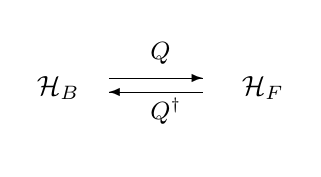
\begin{tikzpicture}
\node at (0.2,0) {$\calH_B$};
\node at (1.5,0) {$\raisebox{.6cm}{\maplr{Q}{Q^\dag}}$};
\node at (2.8,0) {$\calH_F$};
\end{tikzpicture}~.
$$
The Hamiltonian of a superymmstric theory is written as the anti-commutator of supercharges
$$
H:=\{Q,Q^{\dag}\}={ 1\over 2}\left(- {d^2 \over dx^2 }
+ W^\prime(x)^2\right) + {1 \over {2}}\sigma_3W^{\prime\prime}(x)
$$
 In other words, the supercharge is a ``square-root'' of Hamiltonian. In addition one can check that the supercharges commute with the Hamiltonian
\begin{equation}
[H,Q] =[H,Q^{\dag}] = 0 ~. 
\label{susyalg}
 \end{equation}
 
 Let us consider a bosonic eigenstate $|b\rangle \in\calH_B$ of the Hamiltonian
 $$ H |b\rangle =\{Q Q^\dag+Q^\dag Q\}|b\rangle =Q^\dag Q|b\rangle =E|b\rangle~, $$
 for $E>0$. Now its \textbf{superpartner} $|f\rangle =Q|b\rangle$ has  the same energy
 $$  H |f\rangle =\{Q Q^\dag+Q^\dag Q\}Q |b\rangle =Q Q^\dag Q|b\rangle =E|f\rangle~.$$
In a similar fashion, for a fermionic eigenstate $|f\rangle \in\calH_F$ with $E>0$, one can show that its superpartner $|b\rangle =Q^\dag|f\rangle$ has the same energy. In fact, the commutation relation \eqref{susyalg} is
responsible for the degeneracy.


\begin{figure}[h]\centering
\includegraphics{hilbert}
\end{figure}


On the other hands, situation drastically changes for states with $E=0$. For a  bosonic state $|b\rangle$ with zero energy $H|b\rangle=0$, we have $\langle b|Q^\dag Q |b\rangle=0$ so that the supercharge annihilates the state $Q|b\rangle=0$ and therefore there is no fermonic partner. Similarly, for a fermionic state $|f\rangle$, one can show that $Q^\dag |f\rangle$ so that there is no bosonic partner. Since  these zero energy states $|z\rangle$ are annihilated by both supercharges $Q$ and $Q^\dag$, they are invariant under supersymmetric transformation
$$
\exp(i\epsilon Q)|z\rangle=|z\rangle~,\qquad \exp(i\epsilon Q^\dag)|z\rangle=|z\rangle~.
$$
Therefore, they are also called \textbf{supersymmetric states}.



Witten considered the difference between bosonic and fermionic zero energy states \cite{Witten:1982}. To this end, he has introduced the index $\Tr(-1)^F$. Since the excited states do not contribute to the index because there are always boson-fermion pairs. Therefore, the index is equal to
$$
\Tr(-1)^F =\dim \Ker Q- \dim \Ker Q^\dag
$$
Note that the space of bosonic zero energy states can be expressed as $\Ker Q$ whereas the space of fermionic zero energy states can be written as $\Ker Q^\dag$.

Since zero energy sates obey
$$
\left(\frac{d}{dx}\pm W^\prime(x)\right)\phi(x)=0~,
$$
we have
$$
\phi(x)=\textrm{const} \times \exp(\mp W(x))~.
$$
The normalizability condition \eqref{L2} requires $\phi(x)\to 0$ as $|x|\to\infty$.   Suppose that the superpotential $W(x)$ is subject to polynomial growth $W(x)\sim \lambda x^n$ in the region $|x|\gg R$.

\begin{itemize}
\item When $n$ is even, there exists either bosonic or fermionic zero energy states depending on the sign of $\lambda$. Therefore, the index is equal to the sign of $\lambda$.
\item When $n$ is odd, there is no zero energy state because $W(x)$ changes the sign when $x$ moves from $-\infty$ to $\infty$ so that the index is equal to zero. Although the Hamiltonian is supersymmetric, there is no supersymmetric state for a potential of this type. Therefore, supersymmetry is \textbf{spontaneously broken}.
\end{itemize}

As we have seen, the index is independent of the detail of the superpotential $W(x)$ and it depends only on its asymptotic behavior. This is what we have seen in the first lecture.

%
%If $M$ is an even-dimensional,  oriented, spin-manifold with
%spin-bundles $S^{\pm}$ and
%$W$ is a vector bundle with unitary connection $A$ then the
%{\em coupled Dirac operator} is a natural first-order differential operator
%\begin{equation}
%\label{eq:dirac}
%D_A^+ \colon C^\infty(M, E^+) \to C^\infty(M, E^-).
%\end{equation}
%where
%\begin{equation} \label{1.27.9}
%E^+:=  S^+\otimes W,\;\;  E^-:= S^-\otimes W.
%\end{equation}
%If $M$ is compact, the Atiyah-Singer index theorem \cite{AS0, AS1} 
%gives a topological
%formula for the index of $D^+_A$,
%\begin{equation}
%\label{eq:indextheorem}
%\textrm{ind}(D^+_A):= \dim \ker (D^+_A)  - \dim \coker (D^+_A) = 
%\langle \hat A (M) \ch(W),  [M] \rangle.
%\end{equation}
%
%If $M$ is not a spin-manifold, `generalized Dirac operators' can be
%introduced, even though the Dirac operator itself is not
%well-defined. This can be done by observing that $E = E^+\oplus E^-$
%is a {\em Clifford module} (Clifford multiplication is extended to act
%as the identity on $W$) so that a compatible connection on $E$ leads
%to a Dirac operator as before.  If $M$ is not spin, there is an index
%theorem for Dirac operators defined on (hermitian) Clifford modules $E$
%which can be expressed in the form \cite{BerGetVer}
%\begin{equation} \label{eq:2.27.8}
%\ind(D^+_A) = \langle \widehat{A}(M)\ch(W), [M]\rangle
%\end{equation}
%where the notation will be explained below.  The definition is such
%that if $M$ is spin and \eqref{1.27.9} holds, then the {\em relative
%Chern character} $\ch(E/S)$ reduces to $\ch(W)$, the Chern character
%of $W$.
%
%
%
%
%
%\section{Clifford modules and Dirac operators}
%
%
%In the first part of this section we briefly recall the definitions and some basic
%facts about Clifford modules and Dirac operators. We refer the reader to
%\cite{BeGeVe,Duis96,LawMic89} for details. In our exposition we adopt the notations of
%\cite{BeGeVe}.
%
%In the second part of the section we present some examples of Clifford modules, which
%will be used in the subsequent sections.
%
%%---------------------------------------
%\subsection{The Clifford bundle}
%Suppose $(M,g)$ is an oriented Riemannian manifold of dimension $2n$. For any
%$x\in M$, we denote by $C(T^*_xM)=C^+(T^*_xM)\oplus C^-(T^*_xM)$ the Clifford
%algebra of the cotangent space $T_x^*M$, cf. \cite[\S3.3]{BeGeVe}.
%
%The {\em Clifford bundle \/} $C(M)$ of $M$ (cf. \cite[\S3.3]{BeGeVe}) is the
%$\ZZ_2$-graded bundle over $M$, whose fiber at $x\in M$ is $C(T^*_xM)$.
%
%
%The Riemannian metric $g$ induces the Levi-Civita connection $\nabla$ on $C(M)$
%which is compatible with the multiplication and preserves the $\ZZ_2$-grading on
%$C(M)$.
%
%%-----------------
%\subsection{Clifford modules}
%A {\em Clifford module \/} on $M$ is a complex vector bundle $\E$ on $M$ endowed
%with an action of the bundle $C(M)$. We write this action as
%%\[
%%        (a,s) \ \mapsto \ c(a)s, \quad \mbox{where} \quad
%%                        a\in \gc, \ s\in \gme.
%%\]
%
%A Clifford module $\E$ is called {\em self-adjoint \/} if it is endowed with a
%Hermitian metric such that the operator $c(v):\E_x\to\E_x$ is skew-adjoint, for
%any $x\in M$ and any $v\in T_x^*M$.
%
%
%A connection $\nabla^\E$ on a Clifford module $\E$ is called a {\em Clifford
%connection \/} if it is {\em compatible with the Clifford action}, i.e., if for
%any $a\in \gc$ and $X\in\Gamma(M,TM)$,
%\[
%        [\n^\E_X,c(a)] \ = \ c(\n_X a).
%\]
%In this formula, $\n_X$ is the Levi-Civita covariant derivative on $C(M)$, and
%$[\n^\E_X,c(a)]$ denotes the commutator of the operators $\n_X^\E$ and $c(a)$.
%
%
%Suppose $\E$ is a Clifford module and $\calW$ is a vector bundle over $M$. The
%{\em twisted Clifford module obtained from $\E$ by twisting with $\calW$ \/} is
%the bundle $\E\otimes\calW$ with Clifford action $c(a)\otimes1$. Note that the
%twisted Clifford module $\E\otimes\calW$ is self-adjoint if and only if so is
%$\E$.
%
%Let $\n^\calW$ be a connection on $\calW$ and let $\n^\E$ be a Clifford
%connection on $\E$. Then the {\em product connection}
%\begin{equation}\label{E:nEW}
%        \n^{\E\otimes\calW} \ = \ \n^\E\otimes 1 \ + \ 1\otimes \n^\calW
%\end{equation}
%is a Clifford connection on $\E\otimes\calW$.
%
%%------------------------
%\subsection{The chirality operator. The natural grading}
%Let $e_1\nek e_{2n}$ be an oriented orthonormal basis of $C(T_x^*M)$ and
%consider the element
%\begin{equation}\label{E:Gam}
%        \Gamma\ = \ i^n\, e_1\cdots e_{2n} \ \in \ C(T_x^*M)\otimes\CC.
%\end{equation}
%This element is independent of the choice of the basis, anti-commutes with any
%$v\in T_x^*M\subset C(T_x^*M)$, and satisfies $\Gamma^2=-1$, cf.
%\cite[\S3.2]{BeGeVe}. This element $\Gam$ is called the {\em chirality
%operator}. We also denote by $\Gam$ the section of $C(M)$ whose restriction to
%each fiber is equal to the chirality operator.
%
%Let $\E$ be a Clifford module, i.e. (cf. \eqref{clmodule}), a vector bundle over
%$M$ endowed with a fiberwise action of $C(M)$. Set
%\begin{equation}\label{E:grad}
%        \E^\pm \ = \ \{v\in \E: \ \Gam\, v=\pm v\}.
%\end{equation}
%Then $\E=\E^+\oplus\E^-$ is a {\em graded module} over $C(M)$ in the sense that
%$C^+(M)\cdot\E^\pm\subset \E^\pm$ and $C^-(M)\cdot\E^\pm\subset \E^\mp$.
%
%We refer to the grading \eqref{grad} as the {\em natural grading \/} on $\E$.
%Note that this grading is preserved by any Clifford connection on $\E$. Also, if
%$\E$ is a self-adjoint Clifford module (cf. \eqref{clmodule}), then the
%chirality operator $\Gam:\E\to\E$ is self-adjoint. Hence, the subbundles
%$\E^\pm$ are orthogonal with respect to the Hermitian metric on $\E$. {\em In
%this paper we endow all our Clifford modules with the natural grading.}
%
%
%
%
%
%
%
%%-------------------------------
%\subsection{Dirac operators}
%The {\em Dirac operator \/} associated to a Clifford connection $\n^\E$ is
%defined by the following composition
%%\begin{equation}\label{E:dir1}
%%\begin{CD}
%%        \gme @>\n^\E>> \g(M,T^*M\otimes \E) @>c>> \gme.
%%\end{CD}
%%\end{equation}
%In local coordinates, this operator may be written as $D=\sum\,
%c(dx^i)\,\n^\E$. Note that $D$ sends even sections to odd sections and
%vice versa: $D:\, \Gam(M,\E^\pm)\to \Gam(M,\E^\mp)$.
%
%Suppose that the Clifford module $\E$ is endowed with a Hermitian structure and
%consider the $L_2$-scalar product on the space of sections  defined by the
%Riemannian metric on $M$ and the Hermitian structure on $\E$. By
%\cite[Proposition~3.44]{BeGeVe}, {\em the Dirac operator associated to a
%Clifford connection $\n^\E$ is formally self-adjoint with respect to this scalar
%product if and only if $\E$ is a self-adjoint Clifford module and $\n^\E$ is a
%Hermitian connection.}


\begin{thebibliography}{99}
\bibitem{index-book}
Shing-Tung Yau, ed. (2009), \textit{The Founders of Index Theory (2nd ed.)}, Somerville, Mass.: International Press of Boston, ISBN 978-1571461377 - Personal accounts on Atiyah, Bott, Hirzebruch and Singer.


\bibitem{Dai}
Xianzhe Dai, \textit{Lectures on Dirac Operators and Index Theory},

 \href{http://web.math.ucsb.edu/~dai/book.pdf}{ http://web.math.ucsb.edu/dai/book.pdf}

\bibitem{BGV}
Berline Getzler Vergne, \textit{Heat kernels and Dirac operators}, Springer Science \& Business Media, 2003.

\bibitem{Witten:1982}
E.~Witten, \textit{Supersymmetry and Morse theory}, J. diff. geom \textrm{17}.4 (1982): 661-692.



\end{thebibliography}

\end{document}
